%% LyX 2.3.6 created this file.  For more info, see http://www.lyx.org/.
%% Do not edit unless you really know what you are doing.
\documentclass[english,aspectratio=169]{beamer}
\usepackage{lmodern}
\renewcommand{\sfdefault}{lmss}
\renewcommand{\ttdefault}{lmtt}
\usepackage[T1]{fontenc}
\usepackage[latin9]{inputenc}
\setlength{\parskip}{\medskipamount}
\setlength{\parindent}{0pt}
\usepackage{url}
\usepackage{amstext}
\usepackage{amssymb}
\usepackage{graphicx}
\PassOptionsToPackage{normalem}{ulem}
\usepackage{ulem}

\makeatletter

%%%%%%%%%%%%%%%%%%%%%%%%%%%%%% LyX specific LaTeX commands.
\pdfpageheight\paperheight
\pdfpagewidth\paperwidth


%%%%%%%%%%%%%%%%%%%%%%%%%%%%%% Textclass specific LaTeX commands.
% this default might be overridden by plain title style
\newcommand\makebeamertitle{\frame{\maketitle}}%
% (ERT) argument for the TOC
\AtBeginDocument{%
  \let\origtableofcontents=\tableofcontents
  \def\tableofcontents{\@ifnextchar[{\origtableofcontents}{\gobbletableofcontents}}
  \def\gobbletableofcontents#1{\origtableofcontents}
}

%%%%%%%%%%%%%%%%%%%%%%%%%%%%%% User specified LaTeX commands.
\usetheme{CambridgeUS}
\usecolortheme{wolverine}
\hypersetup{}
\usepackage{tikz}
\usepackage{color}
\usepackage{listings}


\makeatother

\usepackage{babel}
\begin{document}
\title[M1]{Ocean heat budget and Sea-Ice Thermodynamics}
\author[Magata J Mangatane]{Magata J Mangatane \\ Department of Oceanography \\University of Cape Town}
\date{SEA3004F}
\makebeamertitle

\section*{Outline}
\begin{frame}{Outline}

\tableofcontents{}
\end{frame}


\section{Recap:Ocean heat budget}
\begin{frame}{1st Law of thermodynamics}

\begin{columns}[t]

\column{8cm}
\begin{itemize}
\item \textbf{\footnotesize{}Earth Energy Budget}{\footnotesize{} - accounting for all energy entering, leaving, and being stored in the Earth system}{\footnotesize\par}
\item \textbf{\footnotesize{}Earth Energy Imbalance}{\footnotesize{} - imbalance between energy received, leaving and stored in the Earth system}{\footnotesize\par}
\item \textbf{\footnotesize{}Thermal Energy}{\footnotesize{} -
the internal kinetic energy of an object or system due to motion of its atoms or molecules}{\footnotesize\par}
\item\textbf{\footnotesize{}Temperature }{\footnotesize{} -
average kinetic energy of molecules in a substance}{\footnotesize\par}
\item\textbf{\footnotesize{}Heat }{\footnotesize{} -
the exchange of thermal energy due to a temperature gradient between systems}{\footnotesize\par}
\item \textbf{\footnotesize{}Ocean Heat budget: }{\footnotesize{}$ Q_t = Q_s + Q_{lw} + Q_{sens} + Q_{latent}$}{\footnotesize\par}
\end{itemize}

\column{5cm}

{\footnotesize{}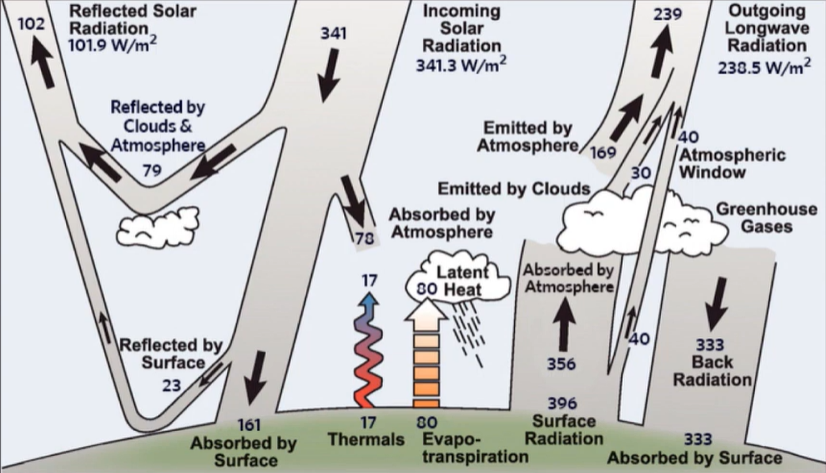
\includegraphics[width=5cm]{../../figures/energy_budget}}{\footnotesize\par}

{\footnotesize{}
\includegraphics[width=5cm]{SEA2004/figures/heat_balance_surface}}{\footnotesize\par}

\end{columns}

\end{frame}

\section{Sea-Ice Thermodynamics}
\begin{frame}{Ocean heat budget and formation of sea ice}

\begin{columns}[t]

\column{8cm}
\begin{itemize}
\item Consider seawater cooling toward its freezing temperature

\item The surface energy budget is given by:
\[
Q_{\text{net}} =
Q_{LW}^{d} +
Q_{SW} -
Q_{LW}^{u} -
Q_{SW}^{a} -
Q_{S+L}
\]

\item If $Q_{\text{net}} < 0$, the ocean loses energy.
\end{itemize}

\column{5cm}

\end{columns}

\end{frame}

\begin{frame}{Ocean heat budget and formation of sea ice}

\begin{columns}[t]

\column{8cm}
\begin{itemize}
\item Consider seawater cooling toward its freezing temperature ($\sim -1.8^\circ$C).

\item The surface energy budget is given by:
\[
Q_{\text{net}} =
Q_{LW}^{d} +
Q_{SW} -
Q_{LW}^{u} -
Q_{SW}^{a} -
Q_{S+L}
\]

\item If $Q_{\text{net}} < 0$, the ocean loses energy.
\end{itemize}

\column{5cm}

{\footnotesize
\hspace*{-1cm} % shifts left by 1 cm
\includegraphics[width=6cm]{../../figures/}
\par}


\end{columns}

\end{frame}

\begin{frame}{Ocean heat budget and formation of sea ice}

\begin{columns}[t]

\column{8cm}
\begin{itemize}
\item Consider seawater cooling toward its freezing temperature ($\sim -1.8^\circ$C).

\item The surface energy budget is given by:
\[
Q_{\text{net}} =
Q_{LW}^{d} +
Q_{SW} -
Q_{LW}^{u} -
Q_{SW}^{a} -
Q_{S+L}
\]

\item If $Q_{\text{net}} < 0$, the ocean loses energy.
\end{itemize}

\column{5cm}

{\footnotesize
\hspace*{-1cm} % shifts left by 1 cm
\includegraphics[width=6cm]{../../figures/}
\par}


\end{columns}

\end{frame}

\begin{frame}{Ocean heat budget and formation of sea ice}

\begin{columns}[t]

\column{8cm}
\begin{itemize}
\item Consider seawater cooling toward its freezing temperature ($\sim -1.8^\circ$C).

\item The surface energy budget is given by:
\[
Q_{\text{net}} =
Q_{LW}^{d} +
Q_{SW} -
Q_{LW}^{u} -
Q_{SW}^{a} -
Q_{S+L}
\]

\item If $Q_{\text{net}} < 0$, the ocean loses energy.
\item If $T_{\text{ocean}} <= -1.8^\circ$C, sea ice forms

\end{itemize}

\column{5cm}

{\footnotesize
\hspace*{-1cm} % shifts left by 1 cm
\includegraphics[width=6cm]{../../figures/}
\par}

\end{columns}

\end{frame}

%conductive heat transfer through sea ice
% Slide 1: Conductive Heat Flux
\begin{frame}{Conductive Heat Flux Through Sea Ice}

\begin{columns}[t]

\column{8cm}
\begin{itemize}
\item Heat is conducted from the relatively warm ocean to the colder ice surface:
\[
F_c = \kappa \frac{\partial T}{h}, \quad \partial T = T_w - T_s
\]
where:
\begin{itemize}
    \item $F_c$ = conductive heat flux (W m$^{-2}$)
    \item $\kappa$ = thermal conductivity of sea ice (W m$^{-1}$ K$^{-1}$)
    \item $\partial T$ = temperature difference across the ice
    \item $h$ = ice thickness
\end{itemize}

\item Note: Flux decreases as ice thickens (\(F_c \propto 1/h\)).

\end{itemize}

\column{5cm}

{\footnotesize
\hspace*{-1cm} % shifts left by 1 cm
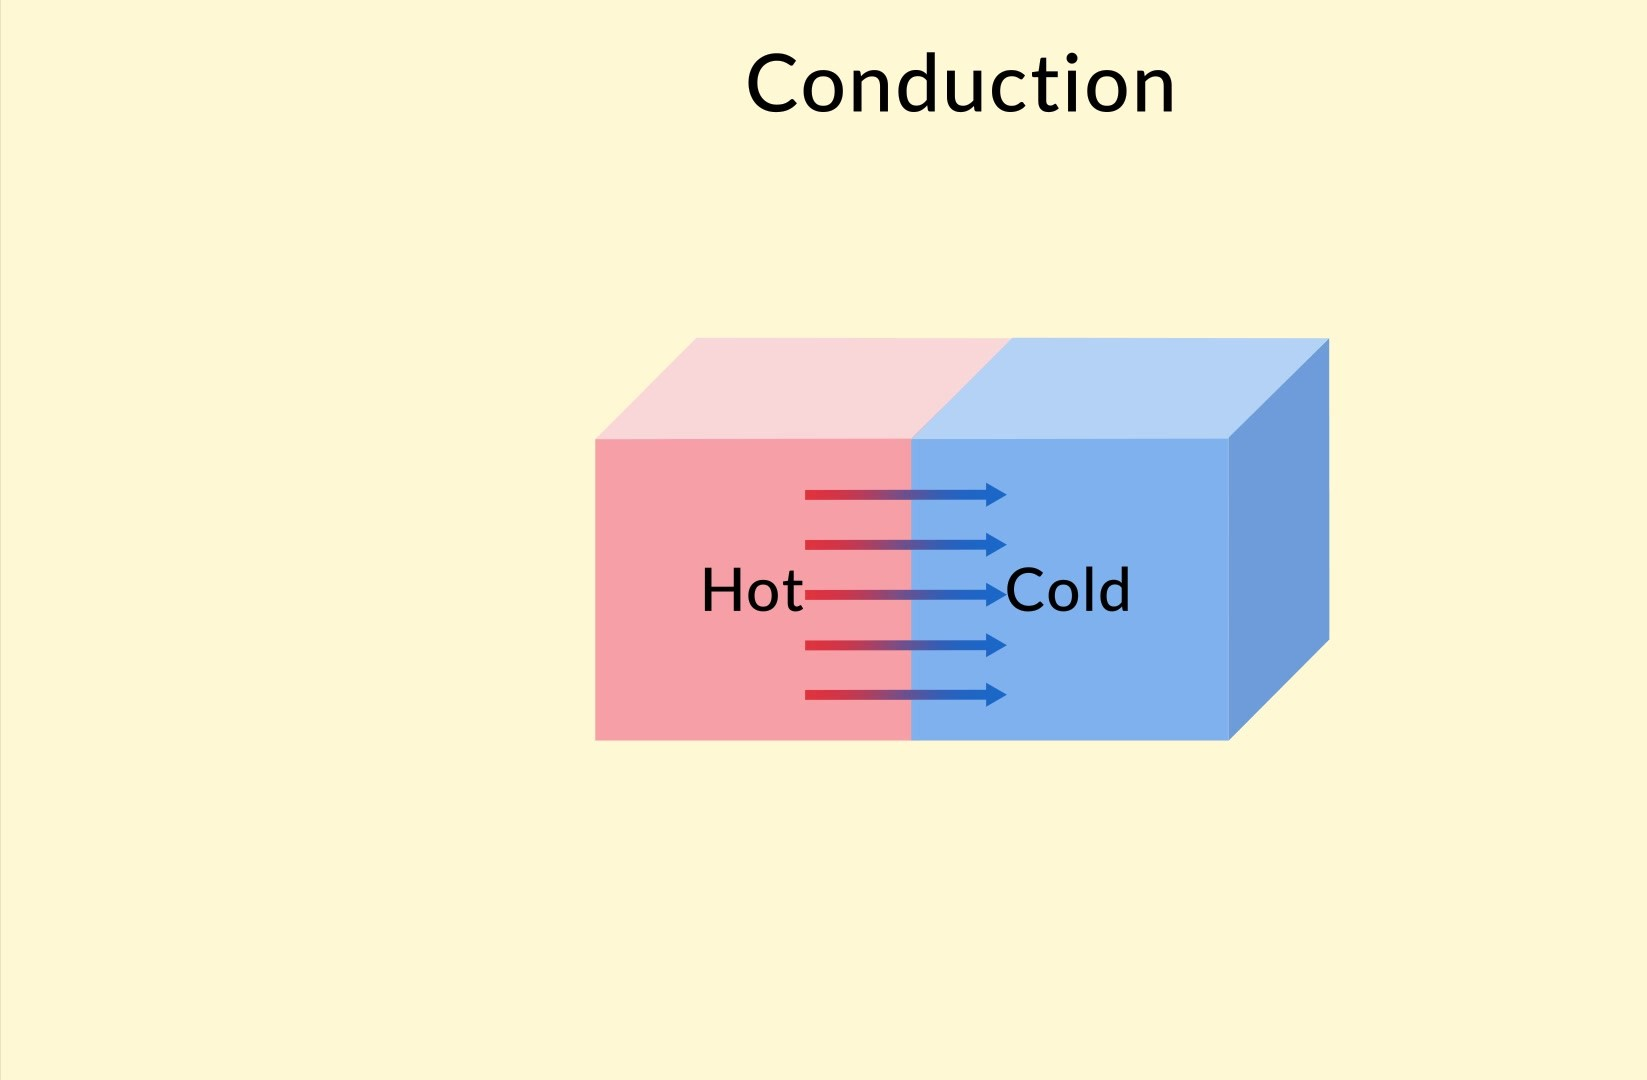
\includegraphics[width=6cm]{../../figures/conduction}
\par
}

\end{columns}

\end{frame}

% Slide 2: Thermal Conductivity
\begin{frame}{Thermal Conductivity of Sea Ice}

\begin{columns}[t]

\column{8cm}
\begin{itemize}
\item Thermal conductivity depends on temperature, salinity, and ice structure:
\[
\kappa = f(T, \text{salinity}, {\text{structure}})
\]

\item Parameterizations:
\begin{itemize}
    \item \textbf{Untersteiner 1971:} Linear model with temperature dependence
    \item \textbf{Pringle et al. 2007:} Updated model accounting for brine volume and temperature variations in multi-year ice
\end{itemize}

\end{itemize}

\column{5cm}

{\footnotesize
\hspace*{-1cm} % shifts left by 1 cm
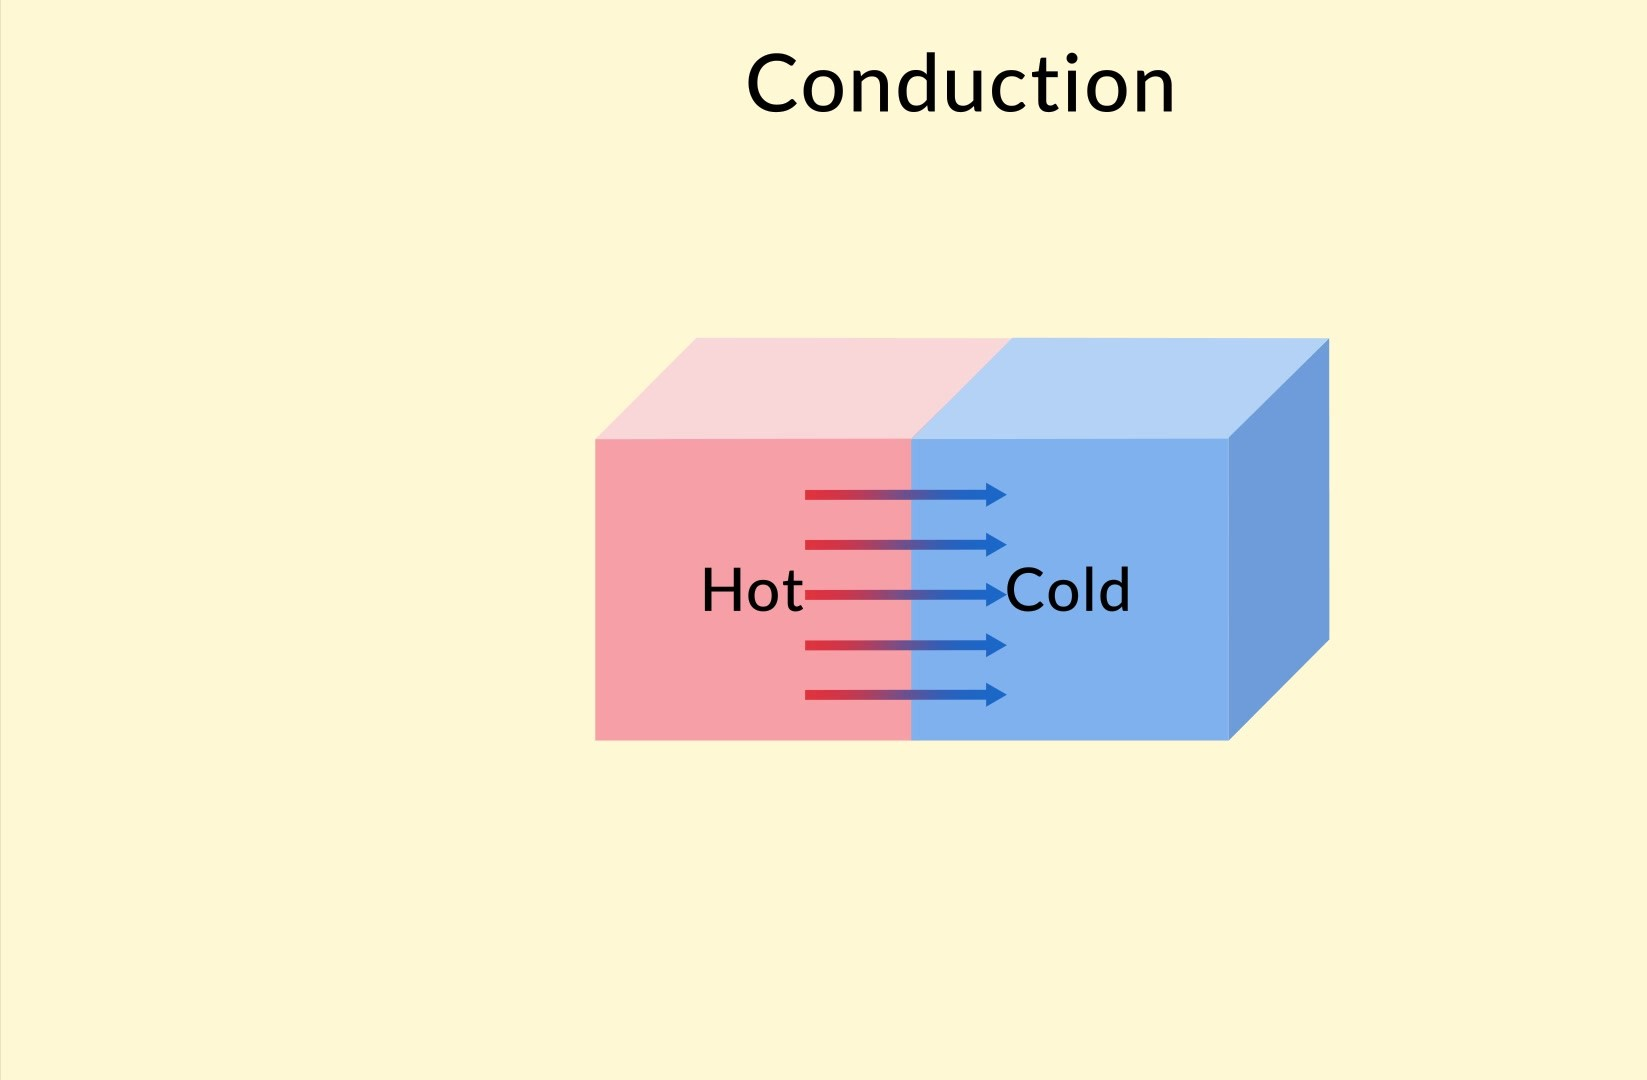
\includegraphics[width=6cm]{../../figures/conduction}
\par
}

\end{columns}

\end{frame}

%end of conductive heat transfer
%dynamics
\section{Sea-Ice Dynamics}
% Slide 1: Sea Ice Momentum Equation
\begin{frame}{Advection of Sea Ice: Momentum Conservation}

\begin{columns}[t]

\column{8cm}
\begin{itemize}
\item Sea ice motion is governed by the conservation of momentum:
\[
m \ \frac{\partial \mathbf{u}}{\partial t} \
= \mathbf{\tau}_a + \mathbf{\tau}_w + \mathbf{F}_i + \mathbf{F}_c + m g \nabla H
\]
where:
\begin{itemize}
    \item $m$ = mass of ice per unit area
    \item $\mathbf{u}$ = ice velocity vector
    \item $\mathbf{\tau}_a$ = wind stress at the ice surface
    \item $\mathbf{\tau}_w$ = ocean stress at the ice bottom
    \item $\mathbf{F}_i$ = sea ice internal stress (from ridging and rafting)
    \item $\mathbf{F}_c$ = Coriolis force
    \item $m g \nabla H$ = gravitational force (for slopes / sea surface tilt)
\end{itemize}

\item The left-hand side represents the change in ice momentum (advection term):
\[
m \frac{d \mathbf{u}}{dt} = m \left( \frac{\partial \mathbf{u}}{\partial t} + \mathbf{u} \cdot \nabla \mathbf{u} \right)
\]

\end{itemize}

\column{5cm}

{\footnotesize
\hspace*{-1cm} % shifts left by 1 cm
\includegraphics[width=6cm]{../../figures/}
\par
}

\end{columns}

\end{frame}

% Slide 2: Forces Acting on Sea Ice
\begin{frame}{Forces Driving Sea Ice Motion}

\begin{columns}[t]

\column{8cm}
\begin{itemize}
\item Main forces in the ice momentum balance:
\begin{itemize}
    \item \textbf{Wind stress ($\mathbf{\tau}_a$)}: drives ice in the wind direction, depends on ice roughness
    \item \textbf{Ocean stress ($\mathbf{\tau}_w$)}: drag from currents below the ice
    \item \textbf{Internal ice stress ($\mathbf{F}_i$)}: resists deformation, important in compacted ice
    \item \textbf{Coriolis force ($\mathbf{F}_c$)}: deflects ice to the right in the Northern Hemisphere
    \item \textbf{Gravity / sea surface tilt ($m g \nabla H$)}: drives motion along pressure gradients
\end{itemize}

\item Ice advection results from solving the momentum equation:
\[
\mathbf{u}(x,y,t) = \text{function of all forces and boundary conditions}
\]

\item Numerical sea ice models often simplify using **linear or viscous-plastic rheologies** for internal stress.

\end{itemize}

\column{5cm}

{\footnotesize
\hspace*{-1cm} % shifts left by 1 cm
\includegraphics[width=6cm]{../../figures/}
\par
}

\end{columns}

\end{frame}

%end dynamics

%begin growth cycles
% Slide 1: Thermodynamic vs Dynamic Control
\section{Arctic vs Antarctic sea ice}
\begin{frame}{Sea Ice Evolution: Thermodynamics and Dynamics}

\begin{columns}[t]

\column{8cm}
\begin{itemize}
\item Sea ice evolves through the interplay of:
\begin{itemize}
    \item \textbf{Thermodynamics:} Growth and decay via heat exchange between atmosphere and ocean
    \item \textbf{Dynamics:} Motion and deformation due to wind, currents, and waves
\end{itemize}

\item Ice properties (thermal and mechanical) and ice type (age-dependent) determine the overall ice cover state

\item Arctic vs Antarctic differences:
\begin{itemize}
    \item Geography, atmospheric forcing, ocean stratification → distinct growth cycles
\end{itemize}

\end{itemize}

\column{5cm}

{\footnotesize
\hspace*{-0.8cm}
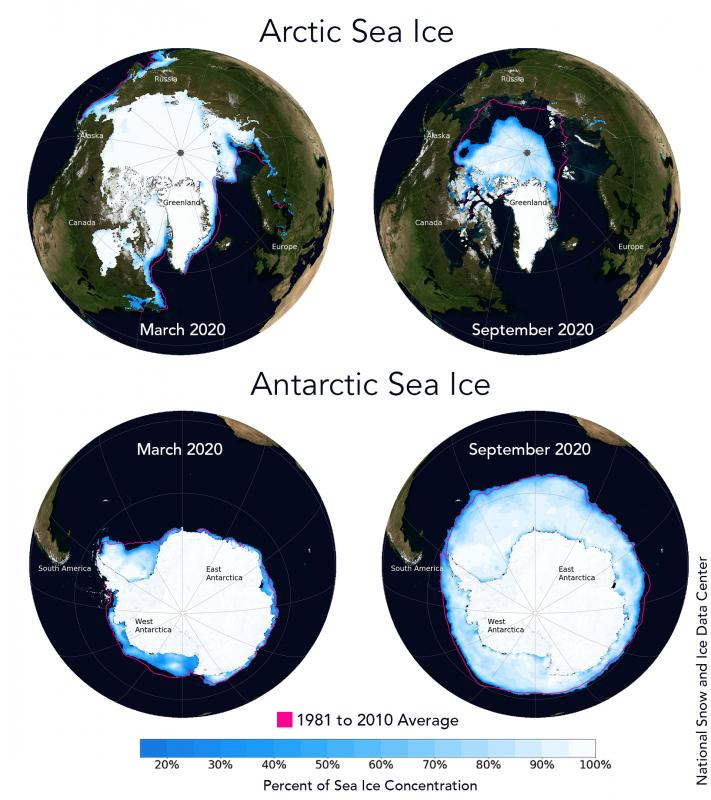
\includegraphics[width=6cm]{../../figures/arctic_vs_antarctic}
\par
}

\end{columns}

\end{frame}

% Slide 2: Arctic Sea Ice: Congelation & Multi-Year Ice
\begin{frame}{Arctic Sea Ice Formation}

\begin{columns}[t]

\column{8cm}
\begin{itemize}
\item Dominated by the \textbf{congelation growth cycle}:
\begin{itemize}
    \item Calm oceans, surface cools to freezing resulting in continuous ice cover
    \item Columnar ice grows from bottom via conduction-limited freezing
\end{itemize}

\item Repeated winter growth + incomplete summer melt favour \textbf{Multi-Year Ice (MYI)}
\begin{itemize}
    \item Survives multiple melt seasons
    \item Stronger mechanical properties, low porosity
\end{itemize}

\item Central Arctic Basin: compact ice pack, weak wave activity

\end{itemize}

\column{5cm}

{\footnotesize
\hspace*{-1cm}
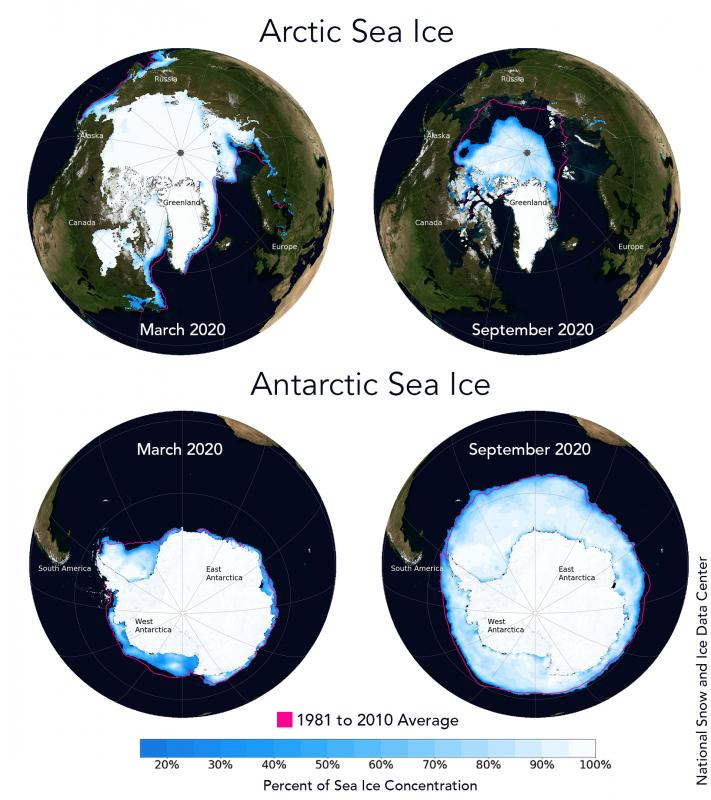
\includegraphics[width=6cm]{../../figures/arctic_vs_antarctic}
\par
}

\end{columns}

\end{frame}

% Slide 3: Antarctic Sea Ice: Pancake Ice
\begin{frame}{Antarctic Sea Ice Formation}

\begin{columns}[t]

\column{8cm}
\begin{itemize}
\item Dominated by the \textbf{pancake ice growth cycle}:
\begin{itemize}
    \item Strong winds and waves favour frazil and grease ice formation
    \item Crystals aggregate into pancake-shaped floes
\end{itemize}

\item Further thickening via:
\begin{itemize}
    \item Bottom congelation growth
    \item Mechanical rafting and deformation
    \item Interstitial ice gluing floes together
\end{itemize}

\item Distinct ice properties:
\begin{itemize}
    \item Granular texture, vertical gradients in salinity & porosity
    \item Contrasts with columnar Arctic ice (stronger, lower porosity)
\end{itemize}

\end{itemize}

\column{5cm}

{\footnotesize
\hspace*{-1cm}
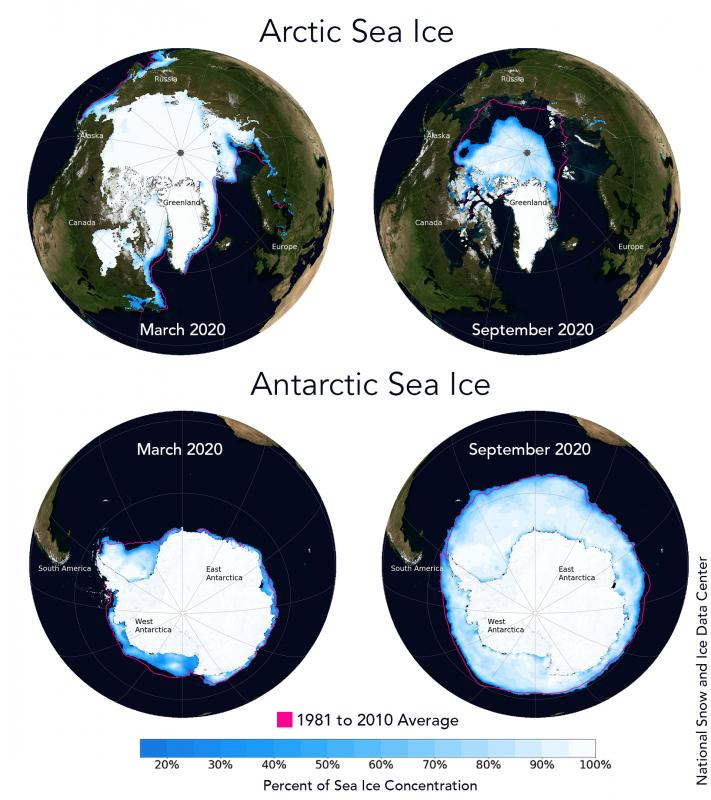
\includegraphics[width=6cm]{../../figures/arctic_vs_antarctic}
\par
}

\end{columns}

\end{frame}


%end growth cycles

\end{document}